%----------------------------------------------------------------------------------------
%	PACKAGES AND THEMES
%----------------------------------------------------------------------------------------
\PassOptionsToPackage{table}{xcolor}
\documentclass[aspectratio=169,xcolor=dvipsnames,svgnames,x11names,fleqn]{beamer}
% \documentclass[aspectratio=169,xcolor=dvipsnames,fleqn]{beamer}

\usetheme{RedVelvet}

\usefonttheme[onlymath]{serif}



\usepackage{xspace}
\usepackage{amsmath}
\usepackage{amssymb}
\usepackage{amsfonts}
\usepackage{color}
\usepackage{physics}
% \usepackage{mathbb}
\usepackage{rahul_math}
\usepackage{bigints}
\usepackage{hyperref}

\usepackage{graphicx} % Allows including images
\usepackage{booktabs} % Allows the use of \toprule, \midrule and \bottomrule in tables
\usepackage{tikz,pgfplots}
\usepackage{subfigure}
\usetikzlibrary{arrows}
\usepackage{minted}
\definecolor{LightGray}{gray}{0.9}
\definecolor{cream}{rgb}{0.92, 0.9, 0.55}
\definecolor{lightblue}{rgb}{0.68, 0.85, 0.9}


\usepackage{xcolor-material}
\usetikzlibrary{fit}
\tikzset{%
apple/.pic={
  \fill [MaterialBrown] (-1/8,0)  arc (180:120:1 and 3/2) coordinate [pos=3/5] (@)-- ++(1/6,-1/7)  arc (120:180:5/4 and 3/2) -- cycle;
  \fill [MaterialLightGreen500] (0,-9/10)  .. controls ++(180:1/8) and ++(  0:1/4) .. (-1/3,  -1) .. controls ++(180:1/3) and ++(270:1/2) .. (  -1,   0) .. controls ++( 90:1/3) and ++(180:1/3) .. (-1/2, 3/4) .. controls ++(  0:1/8) and ++(135:1/8) .. (   0, 4/7)
}
}

\newcommand{\leftdoublequote}{\textcolor{blue}{\scalebox{3}{``}}}

\newcommand{\rightdoublequote}{\textcolor{blue}{\scalebox{3}{''}}}


\usepackage{textcomp}
\usepackage{fontawesome}

\usepackage{overpic}

%----------------------------------------------------------------------------------------
%	TITLE PAGE
%----------------------------------------------------------------------------------------

\usepackage{tikz-qtree,tikz-qtree-compat}
\usetikzlibrary{calc}


\title[CPE 381: Signals and Systems]{CPE 381: Fundamentals of Signals and Systems for Computer Engineers} % The short title appears at the bottom of every slide, the full title is only on the title page
\subtitle{01 Introduction and Preliminaries}

\author[Rahul Bhadani] {{\Large \textbf{Rahul Bhadani}}}

\institute[UAH] % Your institution as it will appear on the bottom of every slide, maybe shorthand to save space
{
    Electrical \& Computer Engineering,  The University of Alabama in Huntsville
}
\date

% \titlegraphic{
%    \includegraphics[width=0.4\linewidth]{figures/UAH_primary.png}
% }

\begin{document}

%-------------------------------------------------
\begin{frame}
  \titlepage
\end{frame}

%-------------------------------------------------
\begin{frame}{Outline}
   \tableofcontents
\end{frame}

%%%%%%%%%%%%%%%%%%%%%%%%%%%%%%%%%%%%%%%%%%%%%%%%%%%%%
\section{Course Logistics}

%-----------------------------------------.-------
\begin{frame}{About Me}
    \begin{columns}[c] % The "c" option specifies centered vertical alignment while the "t" option is used for top vertical alignment

        \column{.60\textwidth} % Left column and width
        \textbf{Rahul Bhadani} \\
        Assistant Professor \\
        Electrical and Computer Engineering \\
        The University of Alabama in Huntsville \\
        Office: 217-H \\
        Email: {\color{MediumRed}{rahul.bhadani@uah.edu}} \\
        Web: {\color{MediumRed}\url{https://rahulbhadani.github.io/}}

        \column{.30\textwidth} % Right column and width
        \includegraphics[width=.89\textwidth]{figures/intro_rkb.jpg}
    \end{columns}
    
    \begin{block}{Research Interests}
    Cyber-physical Systems, Robotics,
    Intelligent Transportation, 
    Connected-and-Autonomous Driving, 
    Applied machine learning,
    Quantum Information Science
    \end{block}
\end{frame}


%-------------------------------------------------

\begin{frame}{Course Logistics}
    \begin{columns}[T] % align columns at the top
    \begin{column}{0.5\textwidth}
        \textbf{Lecture:} \\
        M/W 11:20 AM - 12:40 PM \\
        \vspace{0.3cm}
        \textbf{Location:} \\
        ENG 240 \\
        \vspace{0.3cm}
        \textbf{Prerequisites:}
        \begin{itemize}
        \item EE 213 - Electrical Circuit Analysis I
        \item MA 238 – Applied Differential Equations
        \end{itemize}
    \end{column}
    \begin{column}{0.5\textwidth}
        \textbf{Office Hours:}
        \begin{itemize}
        \item Monday/Wednesday: 1:00 PM - 4 PM
        \end{itemize}
        \textbf{Instructor Email:} rahul.bhadani@uah.edu
    \end{column}
    \end{columns}
\end{frame}

%-----------------------------------------
\begin{frame}{Textbooks}
    \underline{Required:} \emph{\color{DarkGreen}Signals and Systems using Matlab}. Luis F. Chaparro. \par{\color{DarkRed}Elsevier, 3rd Edition, 2019}. \par ISBN: 978-0-12-814204-2, eBook ISBN: 9780128142059\par\vspace{5pt}

        \underline{Suggested Reading:} \textit{Linear Systems and Signals}, B. P. Lathi, Roger Green, Oxford University Press, 2017, 3rd Edition

        \underline{Other Notable Textbooks:}
        \begin{itemize}
            \item Schaum's Outline of Signals and Systems
            \item \textit{Signals and Systems}. Haykin, Simon, and Barry Van Veen. John Wiley \& Sons, 2007.
            \item Asadi, Farzin. Signals and Systems with MATLAB and Simulink. Springer, Dec 2023. ISBN: 9783031456220, 303145622X
        \end{itemize}
\end{frame}

%-----------------------------------------
\begin{frame}{Grading}
\begin{columns}
    \column{0.6\linewidth}

\begin{tabular}{lp{1in} l l l}
\hline
Attendance & 1\%\\\hline
Handwritten Course Notes & 5\%\\\hline
Quizzes & 5\%\\\hline
Classwork & 14\%\\\hline
Homework & 15\%\\\hline
Mid-term Exam 1 & 15\%\\\hline
Mid-term Exam 2 & 15\%\\\hline
Final Exam & 30\%\\\hline
\textbf{Total} & \textbf{100\%}\\\hline
\end{tabular}
\column{0.4\linewidth}
\begin{tabular}{|p{3cm}|p{1.5cm}|}
\hline
\multicolumn{2}{|c|}{\textbf{Grading Scale}} \\ \hline
\textbf{Percentage} & \textbf{Grade} \\ \hline
90\% - 100\% & A \\ \hline
75\% - 89\% & B \\ \hline
60\% - 74\% & C \\ \hline
45\% - 59\% & D \\ \hline
0\% - 44\% & F \\ \hline
\end{tabular}
\end{columns}
\end{frame}


\begin{frame}{Homework Policy}
\begin{itemize}
\item Each late submission will be penalized by 10\% per day for up to 5 days maximum, thereafter, if later, one will receive 0 credit. 
\item Solution to homework will be posted at least 5 days after the due date.
\end{itemize}

\end{frame}

\begin{frame}{Classwork}

\begin{itemize}
\item Each lecture will be followed by in-class problem-solving that students will turn in the same lecture day usually, or the next lecture day, depending on the extent of the work. If you miss the lecture day (either the day it is handed to you, or the day you need to turn in), you will not receive any credit.

\item There will be intermediate small tests to assess your skills based on lectures and the classwork. This portion will count towards your classwork credits.
\end{itemize}



\end{frame}

\begin{frame}{Handwritten Course Notes}

\begin{itemize}
\item You are required to maintain a dedicated course notebook for the course where you will duly record your notes.
\item Handwritten course notes will carry 5\% towards the final grade.

\item Use proper handwriting.

\end{itemize}

\end{frame}

\begin{frame}{Attendance Policy}

\begin{itemize}
\item Must attend all lectures.
\item Attendance will be taken at the middle of the class.
\item Two unexcused absences permitted.
\item No option to make up for classwork.
\end{itemize}

\end{frame}

%-----------------------------------------
\begin{frame}{Exam Schedule}

\definecolor{winemaroon}{HTML}{872341}
\definecolor{coral}{HTML}{E17564}

{\renewcommand{\arraystretch}{1.4}%
\begin{tabular}{|>{\raggedright\arraybackslash}p{3.2cm}|>{\raggedright\arraybackslash}p{5.2cm}|>{\raggedright\arraybackslash}p{4.6cm}|}
\hline
\rowcolor{winemaroon}\multicolumn{3}{|c|}{\textbf{\textcolor{white}{Exam Dates}}}\\\hline
\rowcolor{coral!22}\textbf{Exam} & \textbf{Date} & \textbf{Time}\\\hline
Mid-Term 1 & Monday, September 28, 2026 & 11:20 AM to 12:40 PM\\\hline
Mid-Term 2 & Monday, November 09, 2026 & 11:20 AM to 12:40 PM\\\hline
Final Exam & Friday, December 11, 2026 & 11:30 AM to 2:00 PM\\\hline
\end{tabular}}

\end{frame}

%-----------------------------------------
\begin{frame}{Tentatative Topics}
\small
\begin{itemize}
	\item \color{DodgerBlue4} \underline{Introduction, Mathematical Preliminaries}
 
    \item \color{Firebrick3} \underline{Continuous and Discrete Signals} 
    
    \item  \color{DodgerBlue4} \underline{Linear-time Invariant (LTI) Systems}
    
    \item   \color{Firebrick3} \underline{Laplace Transform}
    
    \item  \color{DodgerBlue4} \underline{Fourier Series for Frequency Analysis} 


    \item  \color{Firebrick3} \underline{Fourier Transform} 
    
    \item \color{DodgerBlue4} \underline{Sampling Theory} 
    \item   \color{Firebrick3}  \underline{Discrete-Time Signals and Systems}
    
    \item  \color{DodgerBlue4} \underline{Z-transform}
    \item  \color{Firebrick3} \underline{Discrete Fourier Analysis} 
   
\end{itemize}
\begin{center}
    Refer to the syllabus for the detailed information on the syllabus.
\end{center}
\end{frame}

%-----------------------------------------
\begin{frame}{In-Class Activity}
  \centering
  \textbf{Introduce Yourself} \\[1em]
  
  \begin{block}{}
    \begin{itemize}
      \item Why Computer Engineering?
      \item What are you hoping to learn from this course?
      \item What is something interesting you did during summer?
    \end{itemize}
  \end{block}

\end{frame}

%%%%%%%%%%%%%%%%%%%%%%%%%%%%%%%%%%%%%%%%%%%%%%%%%%%%%
\section{Motivation}

%-----------------------------------------

\begin{frame}{}
    \begin{center}
    \Huge \bf \color{DarkBlue}
    \faFire
    
    Motivation
\end{center}
\end{frame}

%-----------------------------------------

\begin{frame}{Why Study Signals and Systems}
\centering
    \includegraphics[width=0.4\linewidth]{figures/motivation.png}
\end{frame}

\begin{frame}{We are in digital era}
\centering
    \begin{columns}
          \column{0.33\linewidth}
          \includegraphics[width=0.99\linewidth]{figures/Types-of-Sensors-in-Auto-Pilot.jpg}
         \column{0.33\linewidth}
          \includegraphics[width=0.99\linewidth]{figures/EarthSat_HD.jpg}
          \column{0.33\linewidth}
          \includegraphics[width=0.99\linewidth]{figures/avsensors.png}
    \end{columns}
\end{frame}


\begin{frame}{Sensors and Mobile Devices}
\centering
    \begin{columns}
          \column{0.66\linewidth}
          \includegraphics[width=0.99\linewidth]{figures/Types-of-Sensors-Image-2.jpg}
         \column{0.33\linewidth}
          \includegraphics[width=0.6\linewidth]{figures/iphone.png}
    \end{columns}
\end{frame}

\begin{frame}{Cyber-physical Systems}
\centering
    \begin{columns}
          \column{0.45\linewidth}
          \centering
          \includegraphics[width=0.99\linewidth]{figures/CPS1.png}
          Connected and Autonomous Vehicles
         \column{0.55\linewidth}
         \centering
          \includegraphics[width=0.99\linewidth]{figures/CSP2.png}
          Microgrid
    \end{columns}
\end{frame}

\begin{frame}{Signals in Nature}
    \begin{center}
        Everything in nature is analog and continuous. We use hardware/software interfaces to digitize them, extract information, make inferences, and send them back to the user.
        \includegraphics[width=0.95\linewidth, trim=0 0 0 4cm,clip]{figures/signals_comm.pdf}

    \end{center}
\end{frame}

\begin{frame}{Sampling continuous time signals}
\centering
    \includegraphics[width=0.5\linewidth, trim=0 0 0 0cm,clip]{figures/sampled_sine_wave.png} 
    
    $x[n] = x(nT_s)$,
$T_s$ = sample time.
    
    \tiny
    Code for the figure: \url{https://github.com/rahulbhadani/CPE381_FA26/blob/main/Code/Ch01_sampled_sine_wave.m}
\end{frame}

\begin{frame}{Inherent Discrete Time Signals}
    \begin{center}
         \textbf{Nature may be continuous but human activities naturally lead to some discrete time signals.} 
    \end{center}
   
    
    Examples:
    \begin{itemize}
        \item Stock market closing data
        \item Adaptive cruise control states
        \item Thermostat setpoints
    \end{itemize}
\end{frame}

%%%%%%%%%%%%%%%%%%%%%%%%%%%%%%%%%%%%%%%%%%%%%%%%%%%%%
\section{Course at A Glance}
\begin{frame}{}
    \begin{center}
    \Huge \bf \color{DarkBlue}
    \faGlobe
    
    Course at A Glance
\end{center}
\end{frame}

\begin{frame}{System Thinking}
    \begin{center}
        
    \textbf{System is an abstraction.}
    
    Think of a device or a process as a system -- something that transforms one signal into another.
    
    \centering
      \includegraphics[width=0.65\linewidth,trim=0 0 0 0cm,clip]{figures/system.pdf}

      \end{center}
      
\end{frame}


\begin{frame}{Linear Time-Invariant Systems}


Linearity of a System $\Scal$: \vspace{3pt}

\begin{align*}
\mathcal{S}[a \cdot x(t) + b \cdot y(t)] = \mathcal{S}[a \cdot x(t)] + \mathcal{S}[b \cdot y(t)] = a \cdot \mathcal{S}[x(t)] + b \cdot \mathcal{S}[y(t)]
\end{align*}

Time-invariance of a System $\Scal$: \vspace{3pt}

   If
   \begin{align*}
x(t) \Rightarrow y(t) = \mathcal{S}[x(t)],
\end{align*}

then, the  time-invariance says:
\begin{align*}
x(t \mp \tau) \Rightarrow y(t \mp \tau) = \mathcal{S}[x(t \mp \tau)].
\end{align*}

\textbf{A system satisfying both are Linear Time-Invariant Systems (LTI) Systems.}


\end{frame}


\begin{frame}{Rectangular pulse and Unit impulse}

\begin{columns}
    \column{0.7\linewidth}
    \begin{itemize}
        \item  A rectangular pulse of duration $\Delta$ and unit area:
        \begin{equation*}
            \begin{aligned}
                p_\Delta(t)= \begin{cases}
                    \cfrac{1}{\Delta},\quad -\Delta/2 \leq t \leq \Delta/2\\
                    0, \quad \textrm{otherwise}
                \end{cases}
            \end{aligned}
        \end{equation*}
        \item Unit Impulse:
        \begin{equation*}
            \delta(t) = \lim_{\Delta \to 0}p_\Delta (t)
        \end{equation*}
    \end{itemize}
    \column{0.3\linewidth}
\includegraphics[width=0.7\linewidth,trim=0 0 0 0cm,clip]{figures/unitpulse.png}
\end{columns}
\end{frame}


\begin{frame}{All Signals can be Written Using $\delta
$ Function}
If we do integration in terms of variable $\tau$, we get a generic representation of signals in terms of impulse and shifted impulse.
\begin{columns}
    \column{0.45\linewidth}
    $x(t) = \int_{-\infty}^\infty x(\tau ) \delta(t-\tau)d\tau $

        \includegraphics[width=0.85\linewidth,trim=0 0 0 0cm,clip]{figures/signal_multiplication.png}

    \column{0.55\linewidth}
    \includegraphics[width=0.85\linewidth,trim=0 0 0 0cm,clip]{figures/signal_sums.png}
        \begin{itemize}
            \item Approximation of $x(t)$:
            \footnotesize
            {
            \begin{equation*}
                x_\Delta(t) = \sum_{-\infty}^\infty x_\Delta(t-k\Delta) = \sum_{-\infty}^\infty x(k\Delta) p_\Delta(t-k\Delta)\Delta
            \end{equation*}
            }
        \end{itemize}
\end{columns}
In the limit as $\Delta \to 0$ these pulses become impulses, separated by an infinitesimal value:

$\lim_{\Delta \to 0 }x_\Delta(t) \to x(t)  =  \int_{-\infty}^\infty x(\tau ) \delta(t-\tau)d\tau $
    
\end{frame}

\begin{frame}{Representation of Dynamic Systems}
Dynamic systems can be represented by ordinary differential equations (ODE) with constant coefficients:
\small
\begin{equation*}
\begin{aligned}
    a_n \frac{d^n y(t)}{dt^n} + & a_{n-1} \frac{d^{n-1} y(t)}{dt^{n-1}} + \cdots + a_1 \frac{dy(t)}{dt} + a_0 y(t) = \\
   &  b_m \frac{d^m x(t)}{dt^m} + b_{m-1} \frac{d^{m-1} x(t)}{dt^{m-1}} + \cdots + b_1 \frac{dx(t)}{dt} + b_0 x(t)
\end{aligned}
\end{equation*}
with $n$ initial conditions, $x(t) = 0$ for $t < 0$.

\bf
\begin{center}
    This equation represents a linear ordinary differential equation with constant coefficients, where $ y(t)$  is the output,  $x(t)$  is the input, and  $a_i$  and  $b_i$  are the constant coefficients. 
\end{center}
\end{frame}

\begin{frame}{Impulse Response}
\small
\begin{tcolorbox}[ enhanced, breakable, colframe=roseRed, colback=white, title=~ ]
Output when a system is presented with a unit-impulse signal is called \textbf{response to an impulse signal}, or in short \textbf{impulse response}.
\end{tcolorbox}


What would we get if we pass $x(t)$ through an LTI system $\Scal$?

\vspace{10pt}

We get

\begin{gradyellow}
    $$
    y(t) = \int_{-\infty}^\infty x(\tau) h (t - \tau)d \tau
    $$
\end{gradyellow}

\begin{columns}
    \column{0.4\linewidth}
    where $h(t)$ is the impulse response. Output is the superposition of the responses of each term in the figure.
    \column{0.6\linewidth}
    \includegraphics[width=0.68\linewidth,trim=0 0 0 0cm,clip]{figures/signal_sums.png}
\end{columns}

\end{frame}


\begin{frame}{Periodic Function’s Fourier Series}


If we consider periodic functions with period $T_0$, such that $x(t) = x(t + T_0)$, then

$$
x(t) = \sum_{-\infty}^\infty X(k) e^{jk\Omega_0 t}, \quad \Omega_0 = 2\pi / T_0
$$

is called \textbf{Fourier Series}.



$$
X(k) = \cfrac{1}{T_0}\int_{t_0}^{t_0 + T_0}x(t)  e^{-jk\Omega_0 t}dt, \quad k = 0, \pm 1 , \pm 2, ...
$$
is \textbf{Fourier coefficients}.
\end{frame}

\begin{frame}{Frequency Response $H(jk\Omega_0)$}
\small


\begin{center}
\textbf{Frequency Response}
    $$H(jk\Omega_0) = \int_{-\infty}^{\infty} h(\tau)e^{-jk\Omega_0\tau}d\tau$$
\end{center}

\textcolor{blue}{The frequency response completely characterizes how an LTI system processes periodic signals!}

\end{frame}

\begin{frame}{Response of LTI Systems to Periodic Signal}
    \begin{multiequation}
        x(t) & = \sum_{k} X_k e ^{jk\Omega_0 t}, \quad \Omega_0 = \cfrac{2\pi}{T_0}
        \end{multiequation}
The output in the steady state, if the impulse response is $h(t)$: 
\begin{multiequation}
    y(t) & = \suminf{k} [X_k H(jk\Omega_0)] e ^{jk\Omega_0 t}
\end{multiequation}
Fourier Coefficients of $y(t)$ is $Y_k = X_k H_k(jk\Omega_0)$.

\end{frame}


\begin{frame}{Aperiodic Signal}

    \begin{itemize}
        \item Aperiodic signal can be thought of as a periodic signal with infinite fundamental frequency.
\item In practice, there are no periodic signals, but they are nice mathematical tools.

    \end{itemize}

    $$
    x(t)  = \lim_{T_0 \to \infty } \tilde{x} (t)
    $$
    
\end{frame}

\begin{frame}{Fourier Transform}
In the limiting case, $T_0 \to \infty$,

\begin{custombox}{Fourier Transform}{Tomato}{Purple}

$$
X(\Omega) = \intinf x(t) e^{-j \Omega t} dt
$$
\end{custombox}

    \begin{custombox}{Inverse Fourier Transform}{Purple}{Tomato}

$$
x(t) = \cfrac{1}{2\pi}\intinf X(\Omega) e^{j \Omega t} d\Omega
$$
\end{custombox}

    
\end{frame}

\begin{frame}{Fourier Transform of Periodic Signals}
If the function is periodic, we know that it can be represented as a Fourier series, i.e.
$$
x(t) = \suminf{k} X_k e^{j\Omega_k t}
$$
where 
$$
X_k = \cfrac{1}{T} \intinf x(t) e^{-j\Omega_k t} dt
$$
From the linearity and frequency-shifting property, we can write
$$
X(\Omega) = \sum_k \Fcal [ X_k e^{j\Omega_k t}] = \sum_k 2\pi X_k \delta(\Omega - \Omega_k)
$$
$\Omega_k = k\Omega_0$.

\end{frame}


\begin{frame}{Two-sided or Bilateral Laplace Transform}
    
    \small
    
\begin{custombox}{Definition}{SpringGreen}{pink}
\Large
\begin{equation}
    F(s) = \Lcal[ f(t) ] = \int_{-\infty}^\infty f(t) e^{-st} dt, \quad s\in \textrm{ROC}
\end{equation}
\end{custombox}

ROC = Region of Convergence, the region in the complex plane (henceforth referred to as $s$ plane, as $s= \sigma + j\Omega$ is a complex number).

\begin{itemize}
    \item $\sigma $ : damping factor;
    \item $\Omega $ : frequency in \texttt{rad/s}.
\end{itemize}

\begin{tblock}{}
We see that in Fourier Transform, a signal is represented as a sum of (weighted) sinusoids. However, in Laplace transform, it is a sum of (weighted) damped sinusoids.
\end{tblock}
    
\end{frame}

\begin{frame}{Inverse Laplace Transform}
    \begin{custombox}{Definition}{Dandelion}{MistyRose}
    \Large
        \begin{equation}
            f(t) = \Lcal^{-1}[F(s)] = \cfrac{1}{2\pi j}\int_{\sigma - j\infty}^{\sigma + j\infty} F(s)e^{st}ds, \quad \sigma \in \textrm{ROC}
        \end{equation}
    \end{custombox}
    The relationship between a function and its Laplace transform can be written as:
    \begin{center}
        \begin{equation}
            f(t) \iff F(s)
        \end{equation}
    \end{center}
    
\end{frame}

\begin{frame}{Transfer Function}
\begin{center}
    For a given system $\Scal$, if $f(t) = h(t)$, then $H(s)$ is called the Transfer Function and characterizes the system in $s$-domain (or frequency domain).
    
    \vspace{20pt}
    
    \definecolor{customPurple}{HTML}{B86B9D}

\begin{tikzpicture}
    % Transfer function block
    \node[draw=customPurple, line width=1.5pt, minimum width=3cm, minimum height=1.5cm] (H) {$H(s)$};
    
    % Input arrow
    \draw[-stealth, thick] (-3,0) -- (H.west) node[midway, above] {$x(t)$};
    
    % Output arrow
    \draw[-stealth, thick] (H.east) -- (3,0) node[midway, above] {$y(t)$};
\end{tikzpicture}

\footnotesize

\begin{custombox}{Transfer Function}{LightSkyBlue1}{Tan1}
    $$
    H(s) = \cfrac{\Lcal[\text{output}]}{\Lcal[\text{input}]} = \cfrac{\Lcal[y(t)]}{\Lcal[x(t)]} = \cfrac{Y(s)}{X(s)}
    $$
    
\end{custombox}
    This function is called \textbf{transfer function} because it transfers the Laplace transform of the input to the output. Just as with the Laplace transform of signals, $H (s)$ characterizes an LTI system by means of its poles and zeros. Thus it becomes a very important tool in the analysis and synthesis of systems.

\end{center}

\end{frame}


\begin{frame}{Modeling Sampled Signal using Impulses}

\footnotesize

    If $\Delta \to 0$, we have a train of impulses. In the limiting conditions, we define the impulse \textbf{sampling function} as

    $$
    \delta_{T_s}(t) = \sum_n\delta(t - nT_s)
    $$
    Thus, the sampled signal is:

    $$
    x_s(t) = x(t)\delta_{T_s}(t)
    $$


    \begin{columns}
\column{0.2\linewidth}
    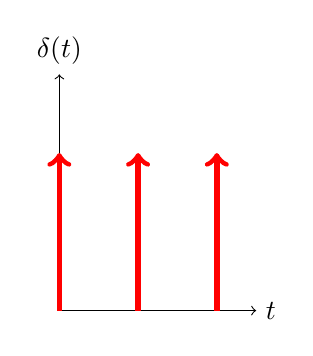
\begin{tikzpicture}
  % Define the pulse width, height, and period
  \def\Deltaval{0.5}
  \def\pulseheight{1/\Deltaval}
  \def\period{1}

  % Draw the x-axis
  \draw[->] (0,0) -- (2.5,0) node[right] {$t$};

  % Draw the y-axis
  \draw[->] (0,0) -- (0,3) node[above] {$\delta(t)$};

  % Draw the pulse train
  \foreach \i in {0,1,2} {
   \draw[thick, ->, red, line width=2pt] (\i,0) -- (\i,\pulseheight);
  }


\end{tikzpicture}

\column{0.1\linewidth}
{
~~~~~\Huge
\faRemove
}

\column{0.2\linewidth}
\includegraphics[width=1.0\linewidth, trim={0cm 0.0cm 0cm 0.0cm},clip]{figures/Sine.pdf}

\column{0.1\linewidth}
{
~~~~~\Huge
\faArrowRight 
}

\column{0.2\linewidth}
{
\includegraphics[width=1.0\linewidth, trim={0cm 0.0cm 0cm 0.0cm},clip]{figures/Discretize_Sine.pdf}

}
\end{columns}
\end{frame}


\begin{frame}{Sampled Signal in Continuous-Time and Discrete-Time}
Two ways to imagine the sampled signal $x_s(t)$:

\vspace{10pt}

\begin{columns}
    \column{0.5\linewidth}
    \textbf{Continuous-Time Version}
$$x_s(t) = x(t) \delta_{T_s}(t)  = \cfrac{1}{T_s}\suminf{k} x(t) e^{jk\Omega_s t}$$

$$
X_s(\Omega) = \cfrac{1}{T_s}\suminf{k} X(\Omega - k\Omega_s)
$$

\column{0.5\linewidth}
\textbf{Discrete-time Version}
$$
x_s(t) = \suminf{n} x(nT_s) \delta(t-nT_s)
$$

$$
X_s(\Omega) = \suminf{n} x(nT_s) e^{-j\Omega T_s n}
$$
\end{columns}
\end{frame}

\begin{frame}{Z-transform from Laplace Transform}
    The discrete equivalent of Laplace Transform that follows:
\begin{itemize}
    \item If the sampled signal is: $x(t) = \sum x(nT_s)\delta(t-nT_s)$
  
    its Laplace transform is : $X(s) = \sum_{n} x(nT_s) \Lcal[\delta(t - nT_s)] = \sum_n x(nT_s) = e^{-ns T_s}$

    \item By letting $z = e^{sT_s}$, 

$$
\Zcal [ x(nT_s)] =\Zcal [ x[n]] = \Lcal[x_s(t)]|_{z = e^{sT_s}} = \sum_{n} x(nT_s) z^{-n} = \sum_{n} x[n] z^{-n}
$$

\textbf{which is called the {\color{red}{Z-transform}} of the sampled signal.}

    
\end{itemize}

\end{frame}

\begin{frame}{Two sided Z-transform}
    Given a discrete-time signal $x[n]$, $ -\infty <n< \infty$, its two-sided Z-transform is given by

    $$
    X(z) = \suminf{n} x[n]z^{-n}
    $$

    defined in a region of convergence (ROC) on the Z-plane.
    
\end{frame}

\begin{frame}{Transfer Function in Z-domain}
    The output $y[n]$ of a causal LTI system is calculated using the convolution sum
    $$
    y[n] = [x*h][n] = \sum_{k = 0}^n x[k]h[n-k] =  \sum_{k = 0}^n h[k]x[n-k]
    $$
    where $x[n]$ is a causal input and $h[n]$ is the impulse response of the system.  Z-transform of the $y[n]$ is the product
    $$
    Y(z) = \Zcal\{ [x*h][n] \} = \Zcal\{ x[n] \} \Zcal\{ h[n] \} = X(z) H(z)
    $$

    and thus the transfer function of a discrete system is defined as

    \begin{gradgreen}
    \begin{center}
        $H(z) = \cfrac{Y(z)}{X(z)}$    
    \end{center}
    \end{gradgreen}
    
\end{frame}

\begin{frame}{The Discrete-Time Fourier Transform (DTFT)}
    For a discrete-time signal $x[n]$, the DTFT is

\begin{gradred}
    \begin{center}
        \begin{multiequation}
        X(e^{j\omega}) = \sum_n x[n] e^{-j \omega n}, \quad -\pi \leq \omega \leq \pi 
    \end{multiequation}
    \end{center}
\end{gradred}

and the inverse DTFT is

   \begin{gradred}
    \begin{center}
         \begin{multiequation}
      x[n] & = \cfrac{1}{2\pi} \int_{-\pi}^\pi  X(e^{j\omega}) e^{j\omega n} d\omega
    \end{multiequation}
    \end{center}
\end{gradred}

\end{frame}

\begin{frame}{Discrete Fourier Transform (DFT)}

\footnotesize

\begin{itemize}
\item In DTFT, the frequency $\omega$ varies from $-\pi$ to $\pi$, so computing $X(e^{j\omega})$ will need to be for uncountable frequencies, not possible for computers.
\item The inverse DTFT requires integration which cannot be exactly implemented in computers.
\end{itemize}
\vspace{5pt}
So we consider Discrete Fourier Transform (DFT) which is computed at discrete frequencies and its inverse also doesn't require integration.

\vspace{5pt}

We can write the DFT of a periodic signal $\tilde{x}[n]$ as 

    \begin{gradred}
       $ X[k] = N\tilde{X}[k] = \sum_{n=0}^{N-1} \tilde{x}[n] e^{-j\omega_0 n k} = \tilde{x}[n] e^{-j2\pi n k/N}, \quad 0\leq k \leq N-1, \omega_0 = 2\pi/N$
    \end{gradred}

    and the inverse DFT is 

    \begin{gradgreen}
       $ \tilde{x}[n] = \cfrac{1}{N}\sum_{k=0}^{N-1}X[k]e^{j2\pi n k/N}, \quad 0\leq n \leq N-1$
    \end{gradgreen}
\end{frame}



\begin{frame}{DFT of Aperiodic Signal}

\footnotesize



\begin{itemize}
\item Consider a discrete signal $y[n]$ of finite length $N$.
\item Choose an integer $L \geq N$, the length of the DFT, to be the fundamental period of a periodic extension $\tilde{y}[n]$ having $y[n]$ as a period with padded zeros if necessary.
\end{itemize}

So, DFT of $\tilde{y}[n]$ is

 \begin{gradred}
 \begin{align*}
 \tilde{y}[n] = \frac{1}{L} \sum_{k=0}^{L-1}\tilde{Y}[k]e^{j2\pi n k / L} \quad 0 \leq n \leq L - 1 
 \end{align*}
 \end{gradred}
 
 and inverse DFT is
 
 \begin{gradgreen}
  \begin{align*}
 \tilde{Y}[k] = \sum_{n=0}^{L-1} y[n]e^{-j 2\pi n k / L} \quad 0 \leq k \leq L - 1
 \end{align*}
 \end{gradgreen}

\end{frame}



\begin{frame}{The Fast Fourier Transform (FFT)}
  \vspace{0.1cm}
  
  \begin{itemize}
    \setlength\itemsep{0.3em} 
    \item FFT efficiently computes the \textbf{DFT}. It is not a new transform.
    \item Utilizes a divide-and-conquer strategy (e.g., Cooley-Tukey algorithm).
    \item Drastically reduces computational complexity:
  \end{itemize}

  \vspace{0.2cm}
  \begin{center}
    {\Large $O(N^2) \quad \longrightarrow \quad O(N \log N)$}
  \end{center}

  \begin{flushright}
    \footnotesize\textit{Makes modern digital signal processing practical.}
  \end{flushright}
  
   \begin{equation*}
    X[k] = \sum_{n=0}^{N-1} x[n] \, W_N^{kn}, \quad \text{where } W_N = e^{-j \frac{2\pi}{N}}
  \end{equation*}

  \vspace{0.05cm}
  
  \begin{equation*}
    X[k] = \underbrace{E[k]}_{\text{even indices}} + W_N^k \underbrace{D[k]}_{\text{odd indices}}
  \end{equation*}


\end{frame}

%-----------------------------------------


\section{Mathematical Preliminaries}

%-----------------------------------------

\begin{frame}{}
    \begin{center}
    \Huge \bf \color{DarkBlue}
    \faCalculator
    
    Mathematical Preliminaries
\end{center}
\end{frame}

%-----------------------------------------
\begin{frame}{Trigonometry}
  \begin{columns}[T]
    \begin{column}{0.5\textwidth}
      \begin{itemize}
        \item \textbf{Sine, Cosine, Tangent:}
          \begin{itemize}
            \item \(\sin(\theta) = \cfrac{\text{p}}{\text{h}}\)
            \item \(\cos(\theta) = \cfrac{\text{b}}{\text{h}}\)
            \item \(\tan(\theta) = \cfrac{\text{p}}{\text{b}}\)
          \end{itemize}
        \item \textbf{Pythagorean Identity:}
          \[
          \sin^2(\theta) + \cos^2(\theta) = 1
          \]
      \end{itemize}
    \end{column}
    \begin{column}{0.5\textwidth}
    \includegraphics[width=0.60\linewidth, trim=2cm 2cm 0 0cm,clip]{figures/pythogoreas.png}
      \begin{itemize}
        \item \textbf{Unit Circle:}
      \end{itemize}
    \end{column}
  \end{columns}
\end{frame}

%-----------------------------------------
\begin{frame}{Trigonometric Identities}
What is the value of $h$ based on the diagram?
    \begin{columns}
        \column{0.3\linewidth}
    \includegraphics[width=0.99\linewidth, trim=2cm 2cm 1cm 1cm,clip]{figures/unit_circle_right_triangle.png}
            \column{0.7\linewidth}
        \begin{itemize}
            \item $\cos\theta =  $
            \item $\sin\theta = $
            \item $\sin(\alpha + \beta) = $
            \item $\cos(\alpha + \beta) = $
            \item $\sin^2(\theta) = $ $\quad\quad\quad\quad\quad\quad\quad$ in terms of $\cos(2\theta)$
            \item $\cos^2(\theta) = $ $\quad\quad\quad\quad\quad\quad\quad$ in terms of $\cos(2\theta)$
            \item $\sin 2\theta = $ $\quad\quad\quad\quad\quad\quad\quad$ in terms of $\theta$
            \item $\cos 2\theta = $ $\quad\quad\quad\quad\quad\quad\quad$ in terms of $\theta$
            \item $\sin (-\theta) = $
            \item $\cos(-\theta) = $
                
            
        \end{itemize}
    \end{columns}
\end{frame}

%-----------------------------------------
\begin{frame}{Trigonometric Identities}
What is the value of $h$ based on the diagram?
    \begin{columns}
        \column{0.3\linewidth}
        \includegraphics[width=0.99\linewidth, trim=2cm 2cm 1cm 1cm,clip]{figures/unit_circle_right_triangle.png}
        \column{0.3\linewidth}
        \begin{itemize} \setlength\itemsep{1.5em}
            \item $\tan(\alpha + \beta) = $

            \item $\tan(\alpha - \beta) = $

            \item $\sin 30^{\circ} = $
            \item $\sin 45^{\circ} = $
            \item $\sin 60^{\circ} = $

            \end{itemize}
\column{0.3\linewidth}
\begin{itemize} \setlength\itemsep{1.5em}
            \item $\cos 30^{\circ} = $
            \item $\cos 45^{\circ} = $
            \item $\cos60^{\circ} = $

            \item $\tan 30^{\circ} = $
            \item $\tan 45^{\circ} = $
            \item $\tan60^{\circ} = $
            
        \end{itemize}
    \end{columns}

    \bigskip

\bf \centering
    What's the range of $\sin \theta$ and $\cos \theta$?
\end{frame}

%-----------------------------------------
\begin{frame}{Trigonometric Functions in Different Quadrant}
\begin{columns}
    \column{0.4\linewidth}
    Four Quadrants:
      
        \includegraphics[width=0.99\linewidth, trim=0cm 0cm 0cm 0cm,clip]{figures/quadrants_plot.pdf}
   \column{0.6\linewidth}
   
Considering a unit circle, in four different quadrants $(x, y)$ signs are different, Hence the trigonometric ratios are also different in signs.

\begin{table}[h!]
\centering
\begin{tabular}{|c|c|c|c|}
\hline
Quadrant & $\sin$ & $\cos$ & $\tan$ \\
\hline
I & + & + & + \\
\hline
II & + & - & - \\
\hline
III & - & - & + \\
\hline
IV & - & + & - \\
\hline
\end{tabular}
\caption{Signs of $\sin$, $\cos$, and $\tan$ in all four quadrants}
\end{table}


\end{columns}
    
\end{frame}

%-----------------------------------------

\begin{frame}{Complex Number}
 \begin{columns}
        \column{0.3\linewidth}
$$z = x +  i y$$
$$ i^2  = -1$$
\includegraphics[width=0.99\linewidth, trim=2cm 2cm 1cm 1cm,clip]{figures/complex_num.pdf}
\column{0.3\linewidth}
Two representations of complex numbers:
$$
z = re^{i\theta}
$$
$$
\text{Conjugate:~~~} \zbar = re^{-i\theta}
$$
\column{0.4\linewidth}
    \begin{itemize}
        \item $ r = \sqrt{x^2 + y^2}$
        \item $\theta = \tan ^{-1} \cfrac{y}{x}$
    \end{itemize}
    Euler's Identity:
    \begin{itemize}\setlength\itemsep{1.0em}
        \item $e^{i\theta} = \cos \theta + i \sin \theta$
        \item $e^{- i\theta} = $
        \item $\cos \theta  = \quad\quad\quad\quad$\\ (in terms of exponential)
        \item $\sin \theta  = \quad\quad\quad\quad$\\ (in terms of exponential)
    \end{itemize}
\end{columns}
\end{frame}

%-------------------------------------------
\begin{frame}{Complex Number}
\begin{columns}
\column{0.4\linewidth}
\textbf{Properties of Conjugates}
\begin{itemize}\setlength\itemsep{1.5em}
    \item $\overline{z + w} = \zbar + \wbar $
    \item$ \overline{zw} = \zbar \wbar$
    \item$ \overline{z^n} = \zbar^n $
    \item $z \zbar =  | z | ^2 $ {\bf \color{red} Prove it!}
\end{itemize}
\column{0.5\linewidth}
{\bf De Moivre’s Theorem}
If $z = r(\cos \theta + i \sin \theta )$ and $n$  is a positive integer, then 
$$
z^n = [ r ( \cos \theta   + i \sin \theta  ) ^n] = r^n  ( \cos n \theta + i \sin n \theta ) 
$$

{\bf Roots of a complex number }
$z = 0$ has $n$ distinct roots:

$$
w_k =  r^{1/n}\bigg[ \cos\bigg( \cfrac{\theta + 2 k \pi }{n} \bigg)  + i \sin\bigg( \cfrac{\theta + 2 k \pi }{n} \bigg)\bigg]
$$

\end{columns}
    
\end{frame}

%-----------------------------------------
\begin{frame}{Complex Exponentials}
We also need to give a meaning to the expression $e^z$ when $z = x + i y $ is a complex number.

Based on the infinite series using Taylor's series expansion for $e^x$, we have

\begin{gradbox}{}
   $$
e^z = \sum_{n = 0}^\infty \cfrac{z^n}{n!} = 1 + z + \cfrac{z^2}{2!}  + \cfrac{z^3}{3!} + \cdots 
$$ 
\end{gradbox}

Can you find out, what should be the value of $e^{iy}$ where $y$ is the real number?

\textbf{Note: } $\cos y = 1 - \cfrac{y^2}{2!} + \cfrac{y^4}{4!} - \cfrac{y^6}{6!}  + \cdots $ and $\quad $ $\sin y =  y - \cfrac{y^3}{3!} + \cfrac{y^5}{5!} - \cdots $

    
\end{frame}


\section{Infinite Series}


\begin{frame}{}
    \begin{center}
    \Huge \bf \color{DarkBlue}
    \faFire
    
    Infinite Series
\end{center}
\end{frame}


\begin{frame}{Sum of an Infinite Sequence}
An infinite series is the sum of an infinite sequence of numbers:
$$a_1 + a_2 + a_3 + \cdots + a_n + \cdots$$
The goal is to understand the meaning of such an infinite sum and develop methods to calculate it.
\end{frame}

\begin{frame}{Partial Sums}
The $n$-th partial sum is:
$$S_n = a_1 + a_2 + a_3 + \cdots + a_n$$
As $n$ gets larger, the partial sums get closer to a limiting value.
\end{frame}

\begin{frame}{Example 1}
Consider the series:
$$1 + \frac{1}{2} + \frac{1}{4} + \frac{1}{8} + \frac{1}{16} + \cdots$$
The partial sums are:
$$S_1 = 1$$
$$S_2 = 1 + \frac{1}{2} = \frac{3}{2}$$
$$S_3 = 1 + \frac{1}{2} + \frac{1}{4} = \frac{7}{4}$$
$$S_n = 1 + \frac{1}{2} + \frac{1}{4} + \cdots + \frac{1}{2^{n-1}} =  \frac{2^n - 1}{2^{n-1}}$$
\end{frame}

\begin{frame}{Convergence of the Series}

$$
S = \lim_{n \to \infty} S_n = \lim_{n\to \infty} \cfrac{2^n - 1}{2^{n-1}} =   \lim_{n \to \infty} \bigg (  \cfrac{2^n}{2^{n-1}} - \cfrac{1}{2^{n-1}}\bigg) =  \lim_{n \to \infty} \bigg( 2 - \cfrac{1}{2^{n-1}}\bigg) = 2
$$

Since the sequence of partial sums converges, the infinite series converges. That is to say:

$$\sum_{n=1}^{\infty} \frac{1}{2^{n-1}} = 2$$
\end{frame}

\begin{frame}{Arithmetic Progression (AP)}
An artihmetic series is of the form: $a, (a+d), (a+2d), \cdots (a+(n-1)d)$.

The sum can be written as:

$$
S_n = a + (a+d)  + (a+2d) + \cdots +(a + (n-1)d) = \cfrac{n}{2}[2a + (n-1)d]
$$

$
a = \text{The first term}
$, $ d = \text{common difference}$.
\end{frame}


\begin{frame}{Geometric Series/Geometric Progression}
A geometric series is of the form: $a, ar, ar^2, \cdots ar^n$.

The sum can be written as:


$$S_n = a + ar + ar^2 + ar^3 + \cdots + ar^n + \cdots = \sum_{n=1}^{\infty} ar^{n-1} = \sum_{n=0}^{\infty} ar^n$$

$
a = \text{The first term}
$, $ r = \text{common ratio}$.


\end{frame}

\begin{frame}{Convergence of Geometric Series}
If $|r| < 1$, the geometric series converges:
$$\sum_{n=1}^{\infty} ar^{n-1} = \frac{a}{1 - r}$$
If $|r| \geq 1$, the series diverges.
\end{frame}

\begin{frame}{Example 2}
Consider the series:
$$\sum_{n=0}^{\infty} (-1)^n \frac{5}{4^n}$$
This is a geometric series with $a = 5$ and $r = -\frac{1}{4}$. Since $|r| < 1$, the series converges:
$$\sum_{n=1}^{\infty} 5 \left(-\frac{1}{4}\right)^{n-1} = \frac{5}{1 - \left(-\frac{1}{4}\right)} = 4$$
\end{frame}

\begin{frame}{Example 3: Telescoping Series}
Find the sum of the telescoping series:
$$\sum_{n=1}^{\infty} \frac{1}{n(n+1)} = \sum_{n=1}^{\infty} \left(\frac{1}{n} - \frac{1}{n+1}\right)$$
The partial sums are:
$$S_n = 1 - \frac{1}{n+1} \to 1 \text{ as } n \to \infty$$
\end{frame}

\begin{frame}{Theorem}
If the series $\sum_{n=1}^{\infty} a_n$ converges, then $\lim_{n \to \infty} a_n = 0$.
\end{frame}

\begin{frame}{Divergence Test}
The series $\sum_{n=1}^{\infty} a_n$ diverges if $\lim_{n \to \infty} a_n$ fails to exist or is different from zero.
\end{frame}

\begin{frame}{Practice Problems}
Determine whether the following series converge or diverge. In the case of convergence, give the sum of the series.
\begin{enumerate}
    \item $\sum_{n=1}^{\infty} \frac{1}{2^n}$
    \item $\sum_{n=1}^{\infty} \frac{n+1}{2n-3}$
    \item $\sum_{n=2}^{\infty} \frac{n^2}{n^2-1}$
    \item $\sum_{n=1}^{\infty} \frac{n(n+2)}{(n+3)^2}$
    \item $\sum_{n=1}^{\infty} \frac{1+2n}{3^n}$
\end{enumerate}
\end{frame}



%-----------------------------------------

\begin{frame}{Derivatives}

\begin{center}
\bf
    Rate of change of a quantity with respect to another quantity.


\par In signals and systems, we are usually interested in the rate of change with respect to time.

$$
f'(t) = \cfrac{df(t)}{dt} = \lim_{h \to 0}\cfrac{f(t+h) - f(t)}{h}
$$

\begin{gradbox}{}
    In computer implementation, $h$ is $\Delta t$. $\Delta t$ is the difference of timestamps between two consecutive samples of a signal. 
\end{gradbox}
\end{center}
\end{frame}

%-----------------------------------------

\begin{frame}{Derivative Review}
 \begin{columns}
\column{0.2\linewidth}
\begin{itemize}
        
    \item $f'(x) = \cfrac{d f(x)}{dx}$
    \item $f'(t) = $
\end{itemize}

\column{0.4\linewidth}
\begin{itemize}
    \item $\frac{d}{dx}(x^n) = nx^{n-1}$
    \item $\frac{d}{dx}(\ln(x)) = \frac{1}{x}$
    \item $\frac{d}{dx}(e^x) = e^x$
    \item $\frac{d}{dx}(\sin(x)) = \cos(x)$
    \item $\frac{d}{dx}(\cos(x)) = -\sin(x)$
    \item $\frac{d}{dx}(\sin^{-1}(x)) = \frac{1}{\sqrt{1 - x^2}}$
    \item $\frac{d}{dx}(\tan(x)) = \sec^2(x)$
    \item $\frac{d}{dx}(\cot(x)) = -\csc^2(x)$
    \end{itemize}


\column{0.4\linewidth}
\begin{itemize}
\item $\frac{d}{dx}(\sec^{-1}(x)) = \frac{1}{x\sqrt{x^2 - 1}}$
    \item $\frac{d}{dx}(\sec(x)) = \sec(x) \tan(x)$
    \item $\frac{d}{dx}(\csc(x)) = -\csc(x) \cot(x)$
    \item $\frac{d}{dx}(\tan^{-1}(x)) = \frac{1}{x^2 + 1}$
    \item $(F \cdot S)' = F \cdot S' + F' \cdot S$
    \item $\left(\frac{N}{D}\right)' = \frac{D \cdot N' - N \cdot D'}{D^2}$
    \item $[f(g(x))]' = f'(g(x)) \cdot g'(x)$
\end{itemize}
\end{columns}
\end{frame}

\begin{frame}{Geometrical Interpretation of Derivatives}
\begin{center}
    \bf
    The derivative $f'(x) $ can be interpreted as the slope of the tangent line at the point $(x,y)$ on the graph of the function  $y = f(x)$.
    \includegraphics[width=0.99\linewidth, trim=0cm 40cm 0cm 0cm,clip]{figures/derivative.pdf}
\end{center}
\end{frame}

\begin{frame}{Geometrical Interpretation of Derivatives}
\begin{center}
    \bf We can use the geometric interpretation \\to help study the behavior and the graph of $f(x)$.
\end{center}
\begin{itemize}
    \item $f'(x) > 0$ exactly when $f(x)$ is increasing.
    \item $f'(x) < 0$ exactly when $f(x)$ is decreasing.
    \item $f'(x) = 0$ exactly when $f(x)$ has a horizontal tangent.
    \end{itemize}
\hrule \vspace{5pt}
\small
In many applications, we want to find local maximum and local minimum values. In these applications, it makes sense to look at the locations on a graph where the slope is $0$. In other words, we often use the following method to find all locations where
the slope of the graph is 0.
\begin{itemize}
    \item Find the formula for the derivative: $f'(x)$.
    \item Set this formula equal to $0$ and solve for $x$.
\end{itemize}
\end{frame}



\begin{frame}{Taylor Series}
\textbf{Function approximation:}
\[
f(x) = f(a) + f'(a)(x-a) + \frac{f''(a)}{2!}(x-a)^2 + \cdots
\]

When $a = 0$, the series is called Maclaurin series.

\textbf{Signal processing examples:}
\begin{align*}
e^x &= 1 + x + \frac{x^2}{2!} + \frac{x^3}{3!} + \cdots \\
\cos(\omega t) &= 1 - \frac{(\omega t)^2}{2!} + \frac{(\omega t)^4}{4!} - \cdots \\
\ln(1+t) &= t - \frac{t^2}{2} + \frac{t^3}{3} - \cdots \quad (|t|<1)
\end{align*}


\end{frame}


\begin{frame}{Taylor Series Applications}
\textbf{Small-angle approximation:} \\
$\sin\theta \approx \theta - \frac{\theta^3}{6}$ for $\theta \ll 1$ \\
Error at $\theta=0.1$ rad: $| \text{Actual} - \text{Approx} | < 0.001\%$

\vspace{20pt}

\textbf{Nonlinear system analysis:} \\
$y(t) = e^{x(t)} \approx 1 + x(t) + \frac{x^2(t)}{2}$ \\
When $x(t) = 0.2\cos(2\pi f t)$, \\
$y(t) \approx 1 + 0.2\cos(2\pi f t) + 0.02\cos^2(2\pi f t)$
\end{frame}



\begin{frame}{Integration}
\begin{center}
    \bf 
    Integration is antiderivative but you can also understand it as an area under the curve. In other words, integration is the summation.
\end{center}

If $\cfrac{d}{dx}F(x) = f(x)$ then $\bigints f(x) dx = F(x)$. 
    
\end{frame}

\begin{frame}{Geometric Interpretation of Integral}
    \begin{center}
        Integral gives the area under a curve
        
        \includegraphics[width=0.29\linewidth, trim=0cm 0cm 0cm 0cm,clip]{figures/integration.pdf}

        $\int_0^1 x^2 dx$
        
    \end{center}
    
\end{frame}


%------------------------------------------------
\begin{frame}{Table of Integrals: Basic Form}

\begin{itemize}
    \item $\int x^n \, dx = \frac{1}{n+1} x^{n+1}$
    \item $\int \frac{1}{x} \, dx = \ln x$
    \item $\int u \, dv = uv - \int v \, du$
    \item $\int u(x)v'(x) \, dx = u(x)v(x) - \int v(x)u'(x) \, dx$
\end{itemize}
    
\end{frame}


\begin{frame}{Table of Integrals: More Functions}
\begin{columns}
    \column{0.5\linewidth}
    \begin{itemize}
    \item $\int \frac{1}{ax + b} \, dx = \frac{1}{a} \ln(ax + b)$
    \item $\int \frac{1}{(x + a)^2} \, dx = -\frac{1}{x + a}$
    \item $\int (x + a)^n \, dx = \frac{(x + a)^{n+1}}{n+1}, \quad n \neq -1$
    \item $\int x(x + a)^n \, dx = \frac{(x + a)^{n+1}(nx + x - a)}{(n+2)(n+1)}$
    \item $\int \frac{dx}{1 + x^2} = \tan^{-1} x$
    \item $\int \frac{dx}{a^2 + x^2} = \frac{1}{a} \tan^{-1} \left(\frac{x}{a}\right)$
    \item $\int \frac{x \, dx}{a^2 + x^2} = \frac{1}{2} \ln(a^2 + x^2)$
    \item $\int \frac{x^2 \, dx}{a^2 + x^2} = x - a \tan^{-1} \left(\frac{x}{a}\right)$
\end{itemize}

\column{0.5\linewidth}
\begin{itemize}
     
    \item $\int \frac{x^3 \, dx}{a^2 + x^2} = \frac{1}{2} x^2 - \frac{1}{2} a^2 \ln(a^2 + x^2)$
    \item $\int e^{ax} = \cfrac{1}{a}e^{ax}$
    \item $\int \sin x dx = -\cos x$
    \item $\int \cos x dx = \sin x$
    \item $\int \tan x dx = -\ln \cos x$
    
\end{itemize}
\end{columns}
\end{frame}

\begin{frame}{Differential Equations}
    \begin{center}
        \bf
        Differential equations are simply equations that have derivatives in them.
    \end{center}
Example:
\begin{itemize}
    \item $\cfrac{dy}{dx} +  5 y = 0$
    \item $y'' + 2y' + 10 y  = 0$
    \item $y'' + 3y' + 2y = 3\cos t$
    
\end{itemize}
    The order of a differential equation is the order of the highest derivative in the equation. They are all examples of `ordinary differential equations'.
\end{frame}


\begin{frame}{Solving Differential Equations}
    Consider 
    $$
    y' = 2y + 3
    $$
    The Fundamental Theorem of Calculus implies $y(t) = \int y'(t) dt$, so we get

    $$
    y(t) = 2\int y(t) dt + 3t + C
    $$
    This is not the closed form and doesn't entirely solve to find a solution $y$. We look at some formula (and their derivation) using the rules of differentiation on how to get a closed-form solution.
\end{frame}

\begin{frame}{Solving Differential Equations}
    The linear differential equation 
    $$
    y' = ay + b
    $$
    with $ a \neq 0, b$ has infinitely many solutions 
    $$
    y(t)= c e^{at}  - \cfrac{b}{a}
    $$
    \bf Proof discussed in class.
    
    \end{frame}

\begin{frame}{Up Next}
\begin{itemize}
    \item Representation of Signals: Continuous and Discrete
    \item Continuous Signals
    \item Using MATLAB
\end{itemize}
    
\end{frame}


%-----------------------------------------
\end{document}